\section{Цель работы}
Построение и анализ фазовых портретов.
\section{Задание на лабораторную работу}
\begin{enumerate}
	\item Изучение фазовых портретов типовых особых точек.
	
	Аналитическим путем исследуйте тип особой точки в положениях равновесия. Постройте фазовый портрет линеаризованной системы.

	Постройте фазовый портрет нелинейной системы для анализа поведения решений в окрестности особых точек и сравните его с фазовым портретом линеаризованной системы.
	\item Построение фазовых портретов для нелинейных систем.
	
	По модели в виде блок-схемы постройте системы дифференциальных уравнений (в математической записи вместо нелинейных блоков можно определить соответствующие функции без их раскрытия).
	\item Построение фазового портрета для маятника.
	
	Постройте фазовый портрет математического маятника, постройте фазовый портрет маятника с учетом вязкого трения.

	В обеих системах проанализируйте поведение системы и особые точки фазового портрета.
	\item Построение фазового портрета осциллятора Ван дер Поля.
	
	Проанализируйте получившийся портрет, оцените влияние параметра $\mu$ на динамику системы.
	\item Построение фазового портрета аттрактора Лоренца (3 порядок) и проанализируйте. Попробуйте изменить параметры и проанализируйте изменения поведения системы.
\end{enumerate}
\section{Основные теоретические положения}

Метод фазовой плоскости дает возможность изобразить качественную картину всей совокупности свободных движений (процессов) 
для выбранной области начальных условий (состояний), а при необходимости — провести точные исследования интересующих типов движений. 
Через каждую точку фазового пространства при условии однозначности функции проходит только одна фазовая траектория. Единственность нарушается в особых точках, соответствующих точкам равновесия. 
Существует несколько основных типов особых точек (типов поведения в окрестности положения равновесия):

\begin{itemize}
	\item устойчивый узел
	\item неустойчивый узел
	\item седло
	\item устойчивый фокус
	\item неустойчивый фокус
	\item центр
\end{itemize}

Заметим также, что особые точки являются частным случаем аттракторов — компактных подмножеств фазового пространства динамической системы, 
все траектории из некоторой окрестности которого стремятся к нему при времени, стремящемся к бесконечности. 
Кроме особых точек (точек равновесия) аттрактором могут быть замкнутые траектории (предельные циклы) или некоторая ограниченная область с неустойчивыми траекториями внутри (как у странного аттрактора).
\subsection{Осциллятор Ван дер Поля}
Осциллятор предложен голландским инженером и физиком Бальтазаром ван дер Полем, во время его работы в компании Philips. 
Ван дер Полем были найдены устойчивые колебания, которые были названы релаксационными, известные как «предельные циклы». 
В сентябре 1927 года Ван дер Поль и его коллега ван дер Марк сообщили, что на определенных частотах были зафиксированы шумы, всегда находящиеся рядом с собственными частотами волн. 
Это было одним из первых наблюдений детерминированного хаоса.

Уравнение Ван дер Поля применяется и в физике, и в биологии. Так, например, в биологии создана модель Фитц Хью-Нагумо. 
Данное уравнение также было использовано в сейсмологии для моделирования геологических разломов

\subsection{Аттрактор Лоренца (3 порядок)}

Аттрактор Лоренца (от англ. to attract — притягивать) ― компактное инвариантное множество $L$ в трехмерном фазовом пространстве гладкого потока, 
которое имеет определенную сложную топологическую структуру и является асимптотически устойчивым, 
оно устойчиво по Ляпунову и все траектории из некоторой окрестности $L$ стремятся к $L$ при $t\,\to\,\infty$ (отсюда название).

\section{Обработка результатов эксперимента}

\subsection{Изучение фазовых портретов типовых особых точек}

\subsubsection{Система 1 - Особая точка \textquotedblleftУстойчивый узел\textquotedblright}

Рассмотрим исходную систему нелинейных дифференциальных уравнений:

$$
\begin{cases}
x' = -4x + 1.4x^2 - 4y \\
y' = 1.5x + y - 2.8y^3
\end{cases}
$$

Проведем линеаризацию, отбросив все нелинейные состаявляющие:

$$
\begin{cases}
x' = -4x - 4y \\
y' = 1.5x + y
\end{cases}
$$

Характеристическая матрица будет иметь вид:

$$
A = 
\begin{pmatrix}
	-4 & -4 \\
	1.5 & 1
\end{pmatrix}
$$

Вычислим её собственные значения:

$$
det(sE - A) = s^2 + 3s + 2
$$

Найдя корни полинома, получим $s_1 = -2$ $s_2 = -1$ - корни действительные отрицательные, 
что соответствует особой точке типа \textquotedblleftустойчивый узел\textquotedblright, 
что соответствует полученному по системе линеаризованных уравнений фазовому портрету (Рис. \ref{fig:1})

\begin{figure}[H]
	\centering
	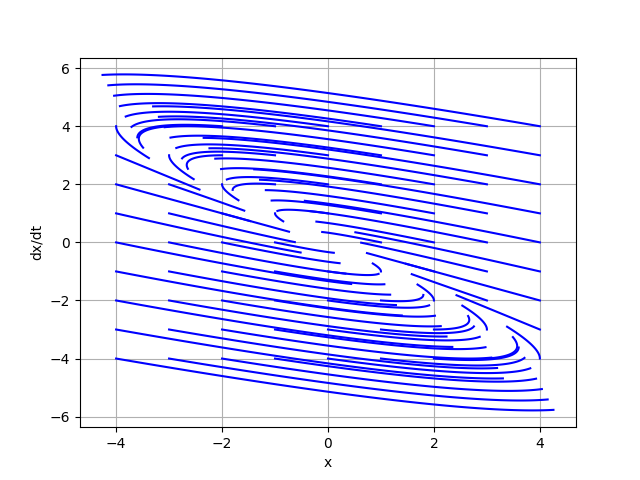
\includegraphics[width=0.6\linewidth]{body/images/Linearized-system-1.png}
	\caption{Фазовый портрет линеаризованной системы 1}
	\label{fig:1}
\end{figure}

При сравнении фазового портрета линеаризованной системы (Рис. \ref{fig:1}) с фазовым портретом 
нелинеаризованной системы (Рис. \ref{fig:2}), можно отметить их схожее поведение в районе нуля.
Отличия траекторий видны на отдалении от данной точки. Точки положения линеаризованной системы
движутся со стороны положительных и отрицательных значений оси $x$, огибают
диагональ и после движутся вдоль неё к точке устойчивости с противоположной стороны.
Точки нелинеаризованной системы же сходятся к нулю со всех сторон

\begin{figure}[H]
	\centering
	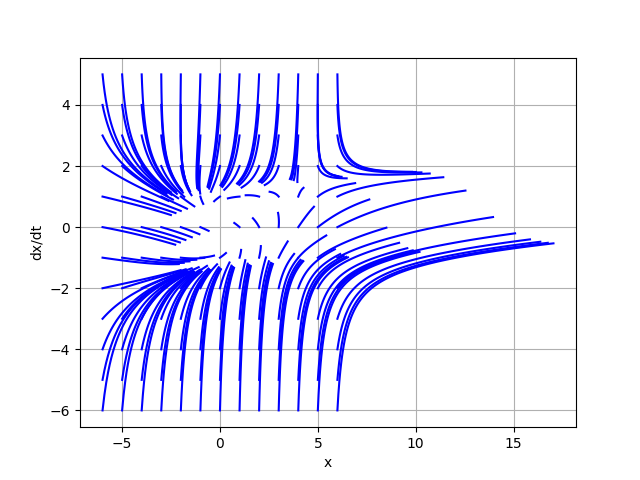
\includegraphics[width=0.6\linewidth]{body/images/System-1.png}
	\caption{Фазовый портрет нелинеаризованной системы 1}
	\label{fig:2}
\end{figure}

\subsubsection{Система 2 - Особая точка \textquotedblleftНеустойчивый узел\textquotedblright}

Рассмотрим исходную систему нелинейных дифференциальных уравнений:

$$
\begin{cases}
x' = x + 0.5y - 1.4y^2 \\
y' = 0.5x - 2.8x^2 + y
\end{cases}
$$

Проведем линеаризацию, отбросив все нелинейные состаявляющие:

$$
\begin{cases}
	x' = x + 0.5y \\
	y' = 0.5x + y
\end{cases}
$$

Характеристическая матрица будет иметь вид:

$$
A = 
\begin{pmatrix}
	1 & 0.5 \\
	0.5 & 1
\end{pmatrix}
$$

Вычислим её собственные значения:

$$
det(sE - A) = s^2 - 2s + 0.75
$$

Найдя корни полинома, получим $s_1 = 1.5$ $s_2 = 0.5$ - корни действительные положительные, 
что соответствует особой точке типа \textquotedblleftнеустойчивый узел\textquotedblright, 
что соответствует полученному по системе линеаризованных уравнений фазовому портрету (Рис. \ref{fig:3})

\begin{figure}[H]
	\centering
	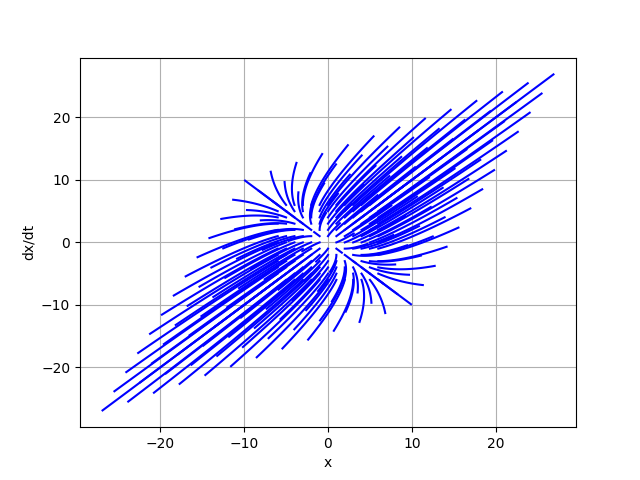
\includegraphics[width=0.6\linewidth]{body/images/Linearized-system-2.png}
	\caption{Фазовый портрет линеаризованной системы 2}
	\label{fig:3}
\end{figure}

При сравнении фазового портрета линеаризованной системы (Рис. \ref{fig:3}) с фазовым портретом нелинеаризованной системы
(Рис. \ref{fig:4}) можно сказать, что траектории линеаризованной системы исходят из начала координат, растягивая
весь свой траекторный массив вдоль наклонной прямой. На фазовой портрете нелинеаризованной системы видно,
что не все траектории исходят из начала координат, а только некоторые. Оставшая же часть, не исходящая из
начала координат, огибает эту самую точку, двигаясь по диагональной прямой

\begin{figure}[H]
	\centering
	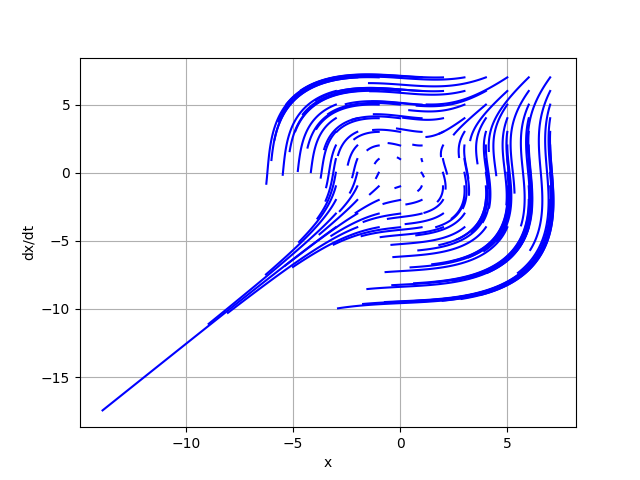
\includegraphics[width=0.6\linewidth]{body/images/System-2.png}
	\caption{Фазовый портрет нелинеаризованной системы 2}
	\label{fig:4}
\end{figure}

\subsubsection{Система 3 - Особая точка \textquotedblleftСедло\textquotedblright}

Рассмотрим исходную систему нелинейных дифференциальных уравнений:

$$
\begin{cases}
x' = 2x +  2.8x^2 + y - 1.4y^2\\
y' = x - 3y
\end{cases}
$$

Проведем линеаризацию, отбросив все нелинейные состаявляющие:

$$
\begin{cases}
	x' = 2x + y \\
	y' = x - 3y
\end{cases}
$$

Характеристическая матрица будет иметь вид:

$$
A = 
\begin{pmatrix}
	2 & 1 \\
	1 & -3
\end{pmatrix}
$$

Вычислим её собственные значения:

$$
det(sE - A) = s^2 + s - 7
$$

Найдя корни полинома, получим $s_{1,2} = \frac{-1\pm\sqrt{29}}{2}$ - корни действительные с разным знаком, 
что соответствует особой точке типа \textquotedblleftседло\textquotedblright, 
что соответствует полученному по системе линеаризованных уравнений фазовому портрету (Рис. \ref{fig:5})

\begin{figure}[H]
	\centering
	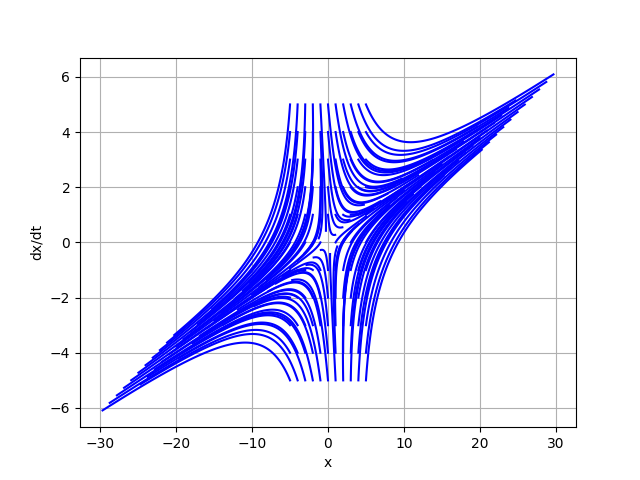
\includegraphics[width=0.6\linewidth]{body/images/Linearized-system-3.png}
	\caption{Фазовый портрет линеаризованной системы 3}
	\label{fig:5}
\end{figure}

При сравнении фазового портрета линеаризованной системы (Рис. \ref{fig:5}) с фазовым портретом нелинеаризованной системы
(Рис. \ref{fig:6}) стоит отметить, что на фазовом портрете линеаризованной системы характерные для \textquotedblleftседла\textquotedblright\ сепаратрисы находятся не ровно перпендикулярно друг относительно друга.
Одна из них, аналогично предыдущей системе, расположена диагонально. Вторая же - вертикально.
На портрете нелинеаризованной системы движение преимущественно горизонтальное, в строну большей координаты,
вертикальное же движение по форме траекторий похоже на песочные часы, с центром в точке $(-2;0)$

\begin{figure}[H]
	\centering
	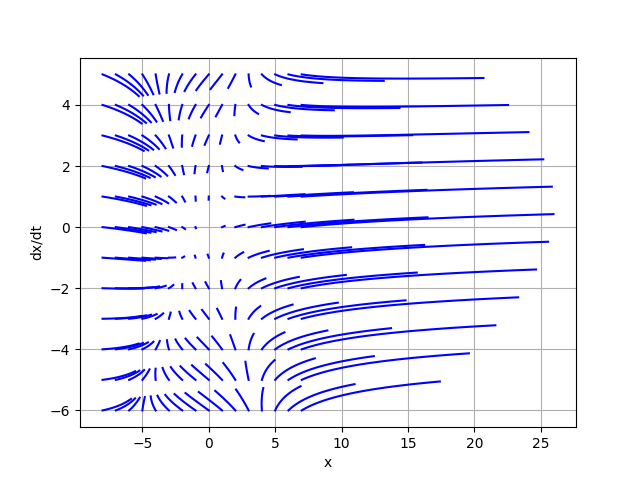
\includegraphics[width=0.6\linewidth]{body/images/System-3.png}
	\caption{Фазовый портрет нелинеаризованной системы 3}
	\label{fig:6}
\end{figure}

\subsubsection{Система 4 - Особая точка \textquotedblleftУстойчивый фокус\textquotedblright}

Рассмотрим исходную систему нелинейных дифференциальных уравнений:

$$
\begin{cases}
x' = - 1.4x^2 + 2y\\
y' = -3x - y
\end{cases}
$$

Проведем линеаризацию, отбросив все нелинейные состаявляющие:

$$
\begin{cases}
	x' = 2y\\
	y' = -3x - y
\end{cases}
$$

Характеристическая матрица будет иметь вид:

$$
A = 
\begin{pmatrix}
	0 & 2 \\
	-3 & -1
\end{pmatrix}
$$

Вычислим её собственные значения:

$$
det(sE - A) = s^2 + s + 6
$$

Найдя корни полинома, получим $s_{1,2} = \frac{-1\pm\sqrt{23}i}{2}$ - корни комплексные с отрицательными действительными частями, 
что соответствует особой точке \textquotedblleftустойчивый фокус\textquotedblright, 
что соответствует полученному по системе линеаризованных уравнений фазовому портрету (Рис. \ref{fig:7})

\begin{figure}[H]
	\centering
	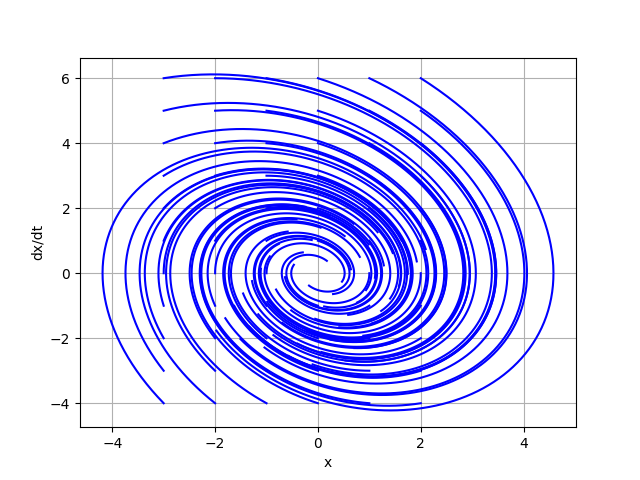
\includegraphics[width=0.6\linewidth]{body/images/Linearized-system-4.png}
	\caption{Фазовый портрет линеаризованной системы 4}
	\label{fig:7}
\end{figure}

При сравнении фазового портрета линеаризованной системы (Рис. \ref{fig:7}) с фазовым портретом нелинеаризованной системы
(Рис. \ref{fig:8}) можно сказать, что линеаризованная система имеет фазовый портрет, похожий на спираль, центр которой
находится в начале координат. Траектории же равномерно покрывают всю радиальную область. Фазовый портрет нелинеаризованной
системы отдалённо напоминает \textquotedblleftзавихрение\textquotedblright\ в начале координат, но большинство траекторий
всё же расходятся, а некоторые огибают \textquotedblleft eye of the storm\textquotedblright

\begin{figure}[H]
	\centering
	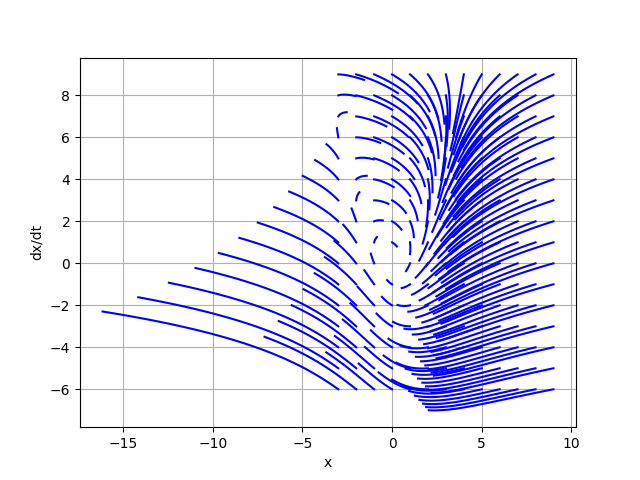
\includegraphics[width=0.6\linewidth]{body/images/System-4.png}
	\caption{Фазовый портрет нелинеаризованной системы 4}
	\label{fig:8}
\end{figure}

\subsubsection{Система 5 - Особая точка \textquotedblleftНеустойчивый фокус\textquotedblright}

Рассмотрим исходную систему нелинейных дифференциальных уравнений:

$$
\begin{cases}
x' = 0.1x - 4y \\
y' = 4x - 2.8x^2 + 0.1y
\end{cases}
$$

Проведем линеаризацию, отбросив все нелинейные состаявляющие:

$$
\begin{cases}
	x' = 0.1x - 4y \\
	y' = 4x + 0.1y
\end{cases}
$$

Характеристическая матрица будет иметь вид:

$$
A = 
\begin{pmatrix}
	0.1 & -4 \\
	4 & 0.1
\end{pmatrix}
$$

Вычислим её собственные значения:

$$
det(sE - A) = s^2 - 0.2s + 16.01
$$

Найдя корни полинома, получим $s_{1,2} = 0.1 \pm 4i$ - корни комплексные с положительными действительными частями, 
что соответствует особой точке \textquotedblleftнеустойчивый фокус\textquotedblright, 
что соответствует полученному по системе линеаризованных уравнений фазовому портрету (Рис. \ref{fig:9})

\begin{figure}[H]
	\centering
	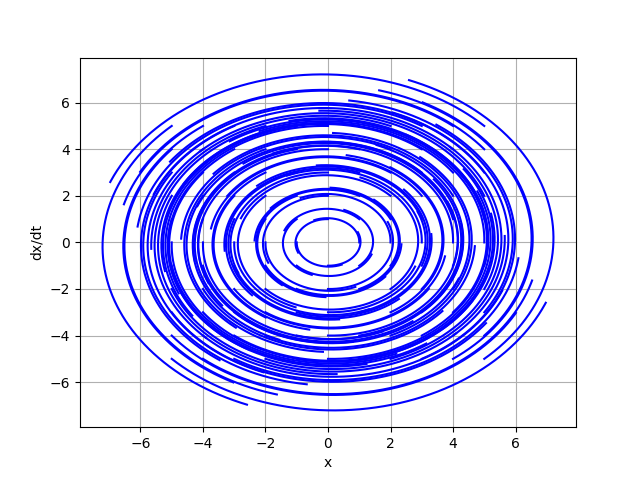
\includegraphics[width=0.6\linewidth]{body/images/Linearized-system-5.png}
	\caption{Фазовый портрет линеаризованной системы 5}
	\label{fig:9}
\end{figure}

При сравнении фазового портрета линеаризованной системы (Рис. \ref{fig:9}) с фазовым портретом нелинеаризованной системы
(Рис. \ref{fig:10}) на первый взляд на портрете видны концентрические неполные окружности, однако, что видно по внешней кривой; 
в разных точках, симметричных относительно начала координат, одной кривой разное расстояние до её центра, что указывает на то, что на самом деле это 
спираль, расходящаяся из центра, но вихрь очень медленно раскручивается. Поведение нелинеаризованной системы соответствует
комбинации особых точек, тем самым образуется \textquotedblleftчереп птицы\textquotedblright, теменная часть которая и соответствует особой точке
\textquotedblleftцентр\textquotedblright, а, непосредственно, клюв представляет собой особную точку \textquotedblleftседло\textquotedblright

\begin{figure}[H]
	\centering
	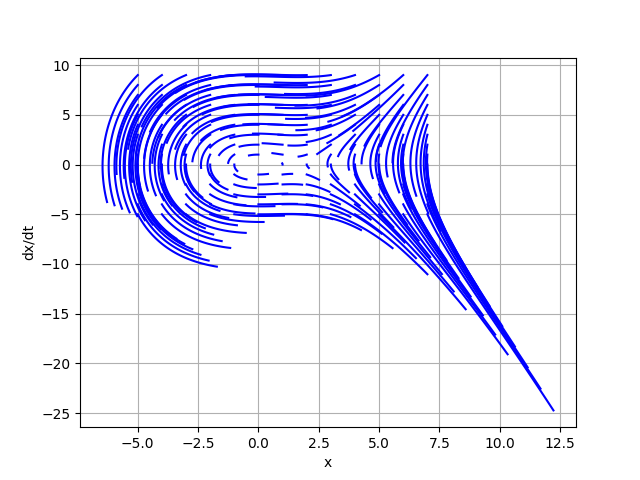
\includegraphics[width=0.6\linewidth]{body/images/System-5.png}
	\caption{Фазовый портрет нелинеаризованной системы 5}
	\label{fig:10}
\end{figure}

\subsubsection{Система 6 - Особая точка \textquotedblleftЦентр\textquotedblright}

Рассмотрим исходную систему нелинейных дифференциальных уравнений:

$$
\begin{cases}
x' = x - 1.4 x^2 - 4y + 4.2y^2\\
y' = 2x + 2.8x^2 - y - 4.2y^3
\end{cases}
$$

Проведем линеаризацию, отбросив все нелинейные состаявляющие:

$$
\begin{cases}
	x' = x - 4y\\
	y' = 2x - y
\end{cases}
$$

Характеристическая матрица будет иметь вид:

$$
A = 
\begin{pmatrix}
	1 & -4 \\
	2 & -1
\end{pmatrix}
$$

Вычислим её собственные значения:

$$
det(sE - A) = s^2 + 7
$$

Найдя корни полинома, получим $s_{1,2} = \pm \sqrt{4}i$ - корни мнимые, 
что соответствует особой точке \textquotedblleftцентр\textquotedblright, 
что соответствует полученному по системе линеаризованных уравнений фазовому портрету (Рис. \ref{fig:11})

\begin{figure}[H]
	\centering
	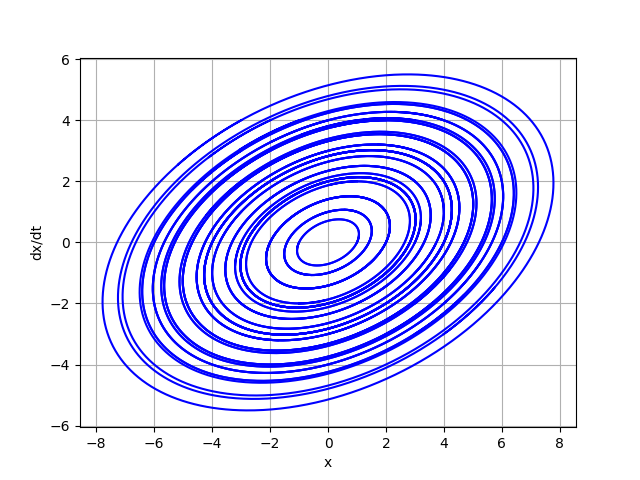
\includegraphics[width=0.6\linewidth]{body/images/Linearized-system-6.png}
	\caption{Фазовый портрет линеаризованной системы 6}
	\label{fig:11}
\end{figure}

При сравнении фазового портрета линеаризованной системы (Рис. \ref{fig:11}) с фазовым портретом нелинеаризованной системы
(Рис. \ref{fig:12}) видно чётко выраженные концентрические эллипсы на фазовом портрете линеаризованной системы.
Портрет нелинеаризованной выглядит намного сложнее, что обусловлено степенями уравнений. Можно отметить, что в отдалении 
основное движение происходит по вертикали, по траекториям, встречающимся у асимптоты, имеющей плавный \textquotedblleftперелом\textquotedblright в районе нуля, 
где можно заметить похожую на особую точку \textquotedblleftустойчивый фокус\textquotedblright часть

\begin{figure}[H]
	\centering
	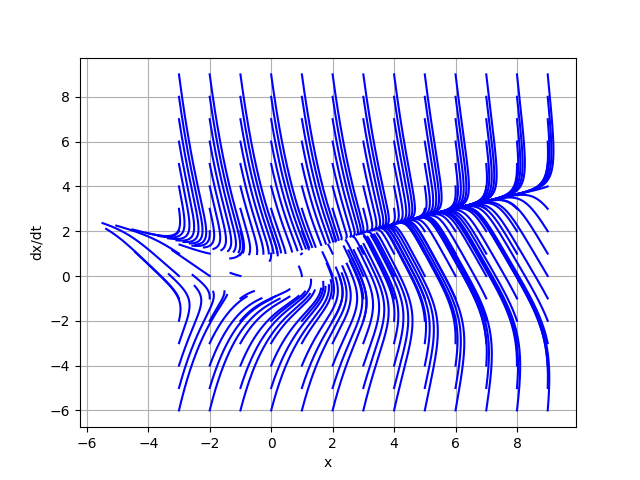
\includegraphics[width=0.6\linewidth]{body/images/System-6.png}
	\caption{Фазовый портрет нелинеаризованной системы 6}
	\label{fig:12}
\end{figure}

\subsection{Построение фазовых портретов для нелинейных систем}

На рис. \ref{fig:13} представлена нелинейная система в виде блок-схемы.

\begin{figure}[H]
	\centering
	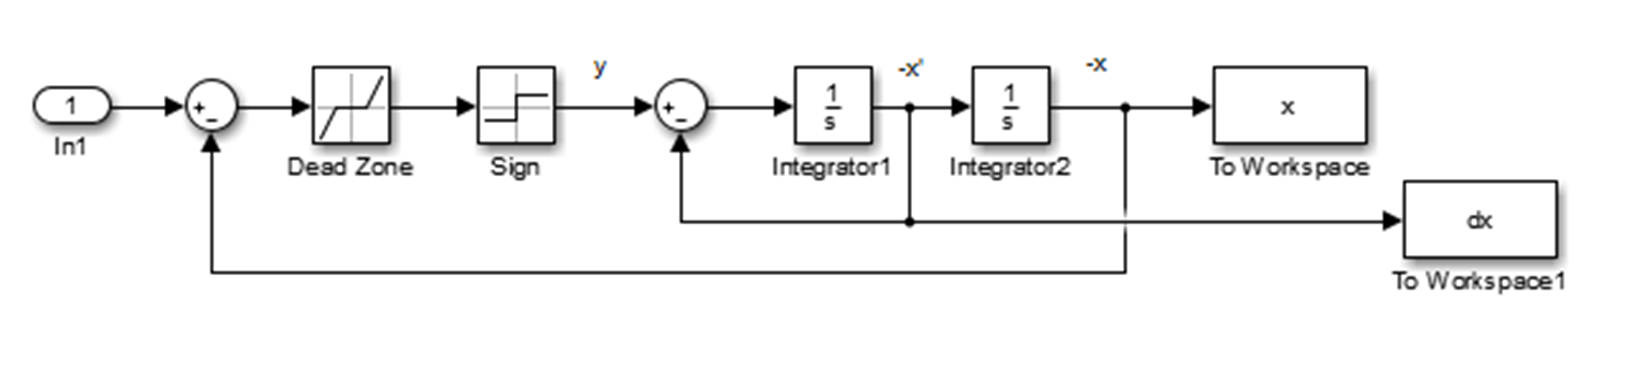
\includegraphics[width=1\linewidth]{body/images/simulink_scheme.png}
	\caption{Нелинейная модель в виде блок-схемы}
	\label{fig:13}
\end{figure}

Обозначим $x'$ и $x''$ как $x_1'$ и $x_2'$ соответственно для большего удобства и избежания путаницы дифференциальности. 
Тогда получим систему уравнений в форме Коши:

$$
\begin{cases}
	x_1' = x_2\\
	x_2' = - x_2 - sign(deadZone(x_1))
\end{cases}
$$

Амплитуда идеального реле: 1

Амплитуда мертвой зоны: 3

\begin{figure}[H]
	\centering
	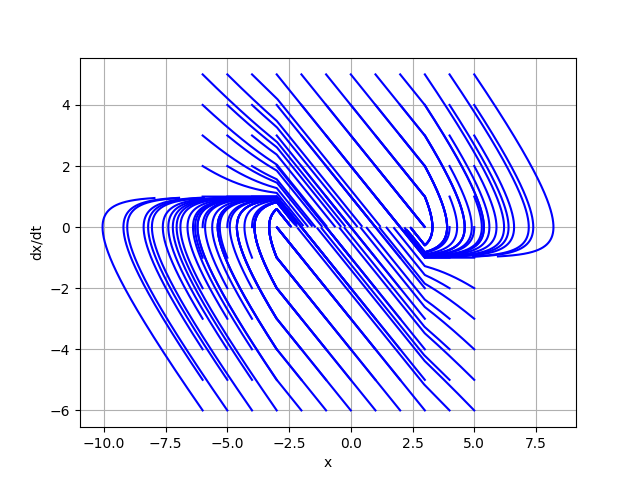
\includegraphics[width=0.7\linewidth]{body/images/Simulink-system.png}
	\caption{Фазовый портрет нелинейной модели}
	\label{fig:14}
\end{figure}

Полученный фазовый портрет полностью схож с особой точкой \textquotedblleftустойчивый узел\textquotedblright, однако точка устойчивости
\textquotedblleftрастянута\textquotedblright по горизонтали на отрезок от $-2.5$ до $2.5$, 
также траектории имеют мгновенные изменения значений координаты, в частности, изменение координаты
$x$ с $-6$ до $-3$ на скорости $x'=1$ и от $6$ до $3$ на скорости $x'=-1$, что соответствует амплитуде реле

\subsection{Построение фазового портрета для маятника}

Математический маятник описывается системой дифференциальных уравнений:

$$
\begin{cases}
{\frac{d \theta}{dt}} = \omega \\ 
{\frac{d \omega}{dt}} = - m g l \sin(\theta)
\end{cases}
$$

Параметры маятника $m$ - масса, $l$ - длинна маятника, $g = 9.81$ - ускорение свободного падения, $b$ - коэффициент трения.
Значения параметров:

\begin{itemize}
	\item $m = 2.8$
	\item $l = 0.357$
	\item $b = 0.31$
\end{itemize}

Фазовый портрет математического маятника с данными параметрами представлен на рис. \ref{fig:15}.
Можно заметить, что фазовый портрет представляет собой повторяющиеся особые точки \textquotedblleftцентр\textquotedblright,
в точках касания которые образуют слияние, которая начинает напоминать особую точку \textquotedblleftседло\textquotedblright

\begin{figure}[H]
	\centering
	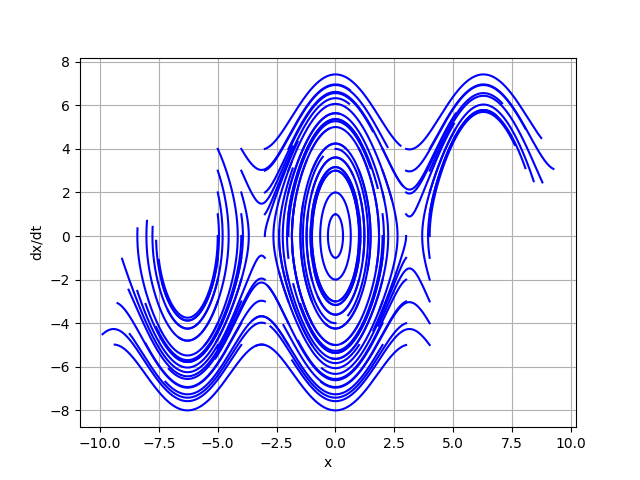
\includegraphics[width=0.7\linewidth]{body/images/Pendulum-system.png}
	\caption{Фазовый портрет маятника}
	\label{fig:15}
\end{figure}

Маятник с учетом вязкого трения:

$$
\begin{cases}
{\frac{d \theta}{dt}} = \omega \\ 
{\frac{d \omega}{dt}} = -b * \omega - m g l \sin(\theta)
\end{cases}
$$

Фазовый портрет маятника с учетом производимого трения представлен на рис. \ref{fig:16}.
На портрете заметно \textquotedblleftнарушение целостности\textquotedblright эллипсов, что очень схоже с устойчивыми фокусами. 

\begin{figure}[H]
	\centering
	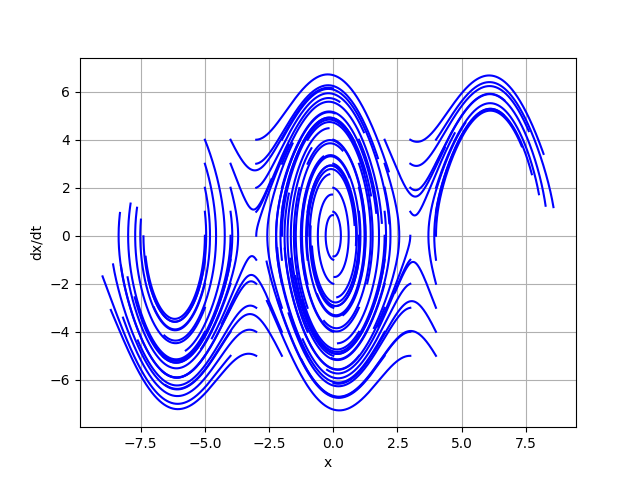
\includegraphics[width=0.7\linewidth]{body/images/Pendulum-system-with-drag.png}
	\caption{Фазовый портрет маятника с учетом вязкого трения}
	\label{fig:16}
\end{figure}

В первом случае, так как рассматривался идеальный математический маятник, особые точки \textquotedblleftцентр\textquotedblright описывали незатухающие колебания,
во втором - колебания с затуханиями, приводящие к постепенному приближению траекторий к нулевой точке.
Так как маятник без трения является идеальным, то никаких искажений не было видно; теперь же явно становятся видны разрывы,
напоминающие \textquotedblleftразрывы 1-го рода\textquotedblright. В целом картина показывает, что особые точки \textquotedblleftцентр\textquotedblright\ 
преобразовываются в особые точки \textquotedblleftустойчивый фокус\textquotedblright. Ранее замкнутые траектории рано или поздно придут в начало координат.
Это будет знамененовать остановку маятника, так как с каждый своим колебанием он теряет долю инерции из-за того самого вязкого трения, которое было учтено.
Без вязкого трения маятник получается идеальным, и, конечно же, никогда не достигнет равновесия, поэтому и фазовый портрет представляет особую точку
\textquotedblleftцентр\textquotedblright, траектории которой никогда не выйдут из замкнутого цикла, дабы достигнуть начала координат

\subsection{Построение фазового портрета осциллятора Ван дер Поля}

Необходимый осциллятор представляется в виде системы дифференциальных уравнений вида

$$
\begin{cases}
{\frac{dx}{dt}} = y \\ 
{\frac{dy}{dt}} = \mu (1-x^2)y-x
\end{cases}
$$

Проведем анализ поведения фазового портрета системы при различных значениях коэффициента $\mu$:
с изначальным $\mu = 14$ (рис. \ref{fig:17}), с $\mu$, уменьшенным в два раза (рис. \ref{fig:18}) и с $\mu$, увеличенным в два раза (рис. \ref{fig:19}).

\begin{figure}[H]
	\centering
	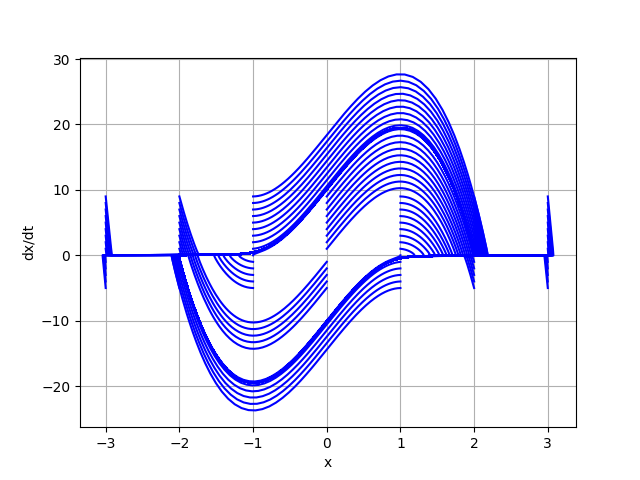
\includegraphics[width=0.6\linewidth]{body/images/Oscillator-with-mu.png}
	\caption{Фазовый портрет осциллятора Ван дер Поля с $\mu=14$}
	\label{fig:17}
\end{figure}

\begin{figure}[H]
	\centering
	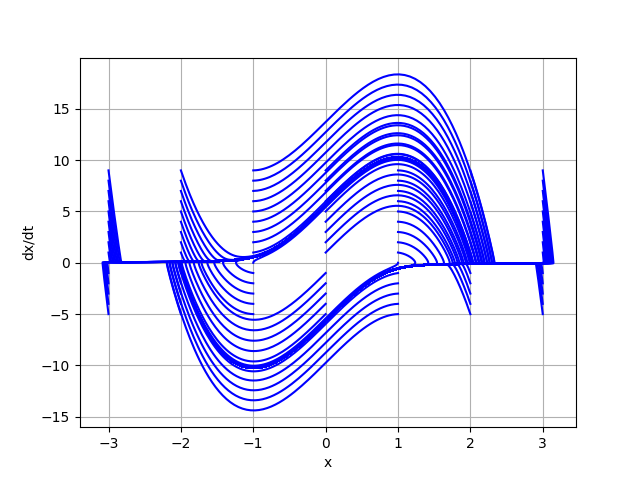
\includegraphics[width=0.6\linewidth]{body/images/Oscillator-with-0.5mu.png}
	\caption{Фазовый портрет осциллятора Ван дер Поля с $\mu=7$}
	\label{fig:18}
\end{figure}

\begin{figure}[H]
	\centering
	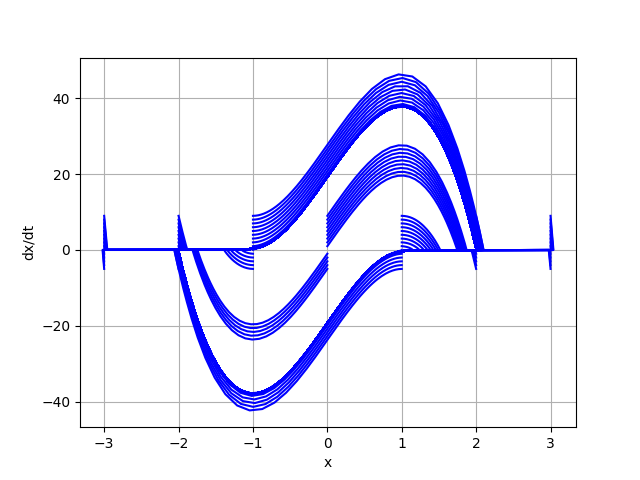
\includegraphics[width=0.6\linewidth]{body/images/Oscillator-with-2mu.png}
	\caption{Фазовый портрет осциллятора Ван дер Поля с $\mu=28$}
	\label{fig:19}
\end{figure}

Полученный портрет похож на период синусоиды, которая имеет \textquotedblleftразрывы 1-го рода\textquotedblright\
в местах, когда траектории пересекают определенное значение по $x$. Формы траекторий ниже нуля полностью зеркально повторяются относительно нуля в положительной полуплоскости.
Можно заметить, что основные линии сгруппированы. Каждая из группированных частей обрывается на своем значении $x$. Плотность этих \textquotedblleft групп \textquotedblright зависит от значения $\mu$ - 
чем оно больше, тем ближе друг к другу отдельные линии траекторий. Также можно наблюдать и влияние величины $\mu$ на значение экстремумов
каждой из траекторий: чем больше значение $\mu$, тем больше экстремум траектории. Сама же форма траекторий очень отдалённо напоминает
форму траектории особой точки \textquotedblleftустойчивый узел\textquotedblright, хотя как таковой выраженной диагонали нет из-за
разрывов

\subsection{Построение фазового портрета аттрактора Лоренца (3 порядок)}

Уравнения для аттрактора задаются уравнениями

$$
\begin{cases}
    \dot x = \sigma (y-x) \\
    \dot y = x (r - z) - y \\
    \dot z = xy - bz
\end{cases}
$$

При следующих значениях параметров: $\sigma = 10$, $r = 28$, $b = 8/3$, $x(0) = 1$, $y(0) = 0$, $z(0) = 0$.
Его фазовый портрет представлен на рис. \ref{fig:20}.

\begin{figure}[H]
	\centering
	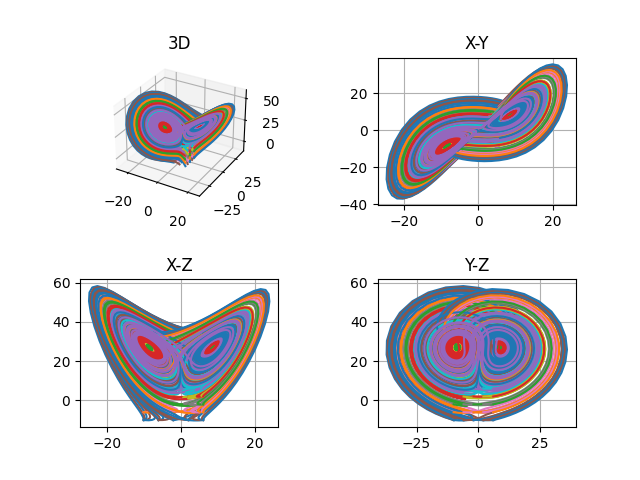
\includegraphics[width=0.7\linewidth]{body/images/Lorenz-attractor-type-1.png}
	\caption{Фазовый портрет аттрактора Лоренца}
	\label{fig:20}
\end{figure}

Портрет схож с двумя \textquotedblleftцентрами\textquotedblright, расположенными близко друг к другу, под определенным углом.

Уменьшим параметр $\sigma$ в 5 раз и построим фазовый портрет системы (Рис. \ref{fig:21}).
Видно, что полученная фигура представляет собой особые точки \textquotedblleftустойчивый фокус\textquotedblright, переплетённые
между собой ещё одной особой точкой - \textquotedblleftседло\textquotedblright, и также расположенные под углом друг к другу

\begin{figure}[H]
	\centering
	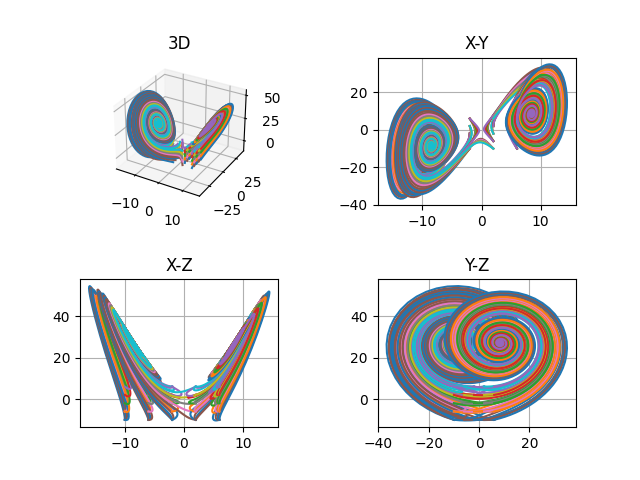
\includegraphics[width=0.7\linewidth]{body/images/Lorenz-attractor-type-2.png}
	\caption{Фазовый портрет аттрактора Лоренца с измененным параметром $\sigma$}
	\label{fig:21}
\end{figure}

Уменьшим параметр $r$ в 7 раз и построим фазовый портрет системы (Рис. \ref{fig:22}).
Благодаря окрашиванию траекторий в разные цвета, становится заметно, что \textquotedblleft центры \textquotedblright стали \textquotedblleft устойчмвыми фокусами \textquotedblright.
Также появляется больше неопределенных траекторий, которые переплетены между собой, в нижней части фигуры

\begin{figure}[H]
	\centering
	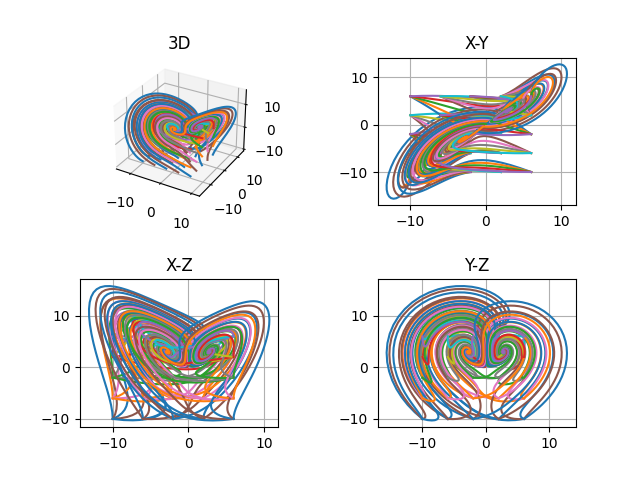
\includegraphics[width=0.6\linewidth]{body/images/Lorenz-attractor-type-3.png}
	\caption{Фазовый портрет аттрактора Лоренца с измененным параметром $r$}
	\label{fig:22}
\end{figure}

Уменьшим параметр $b$ в 4 раз и построим фазовый портрет системы (Рис. \ref{fig:23}). 
Теперь можно увидеть отверстия, что ещё подталкивает к следствию, что фигура является слияние двух особых точек \textquotedblleftцентр\textquotedblright.
При минимально предельном значении параметра $b$, фигура, вероятнее всего, будет образовать собой перекрещивающиеся особые точки
\textquotedblleftцентр\textquotedblright\ с центром в одном и том же месте

\begin{figure}[H]
	\centering
	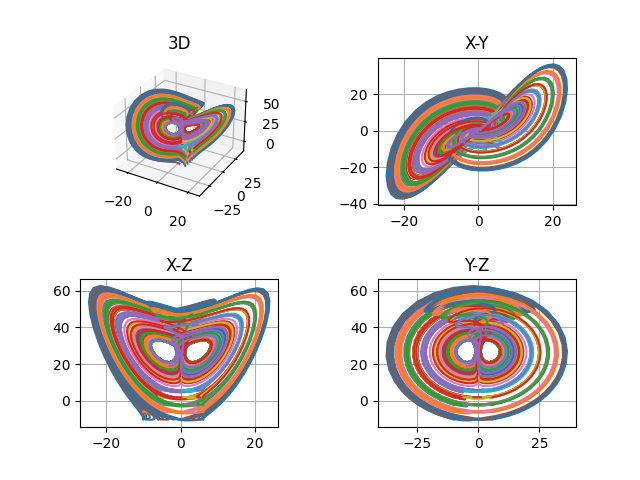
\includegraphics[width=0.6\linewidth]{body/images/Lorenz-attractor-type-4.png}
	\caption{Фазовый портрет аттрактора Лоренца с измененным параметром $b$}
	\label{fig:23}
\end{figure}

\pagebreak
\section{Выводы}
В ходе лабораторной работы были получены фазовые портреты типовых особых точек
путем линеаризации систем, рассмотрено влияние нелинейных звеньев на траектории фазового портрета линейной системы
и проанализировано поведение конкретных систем при различных параметрах: 
маятника, осциллятора Ван дер Поля и аттрактора Лоренца третьего порядка.